\section{Celočíselné programy a relaxácia: dobrý, zlý a škaredý}

\noindent V predchádzajúcich častiach sme ukázali, ako efektívne riešiť úlohu
lineárneho programovania.  Častokrát nás ale zaujímajú iba také riešenia, v
ktorých sú hodnoty nájdených premenných celočíselné. V prvom motivačnom
príklade nám vyšlo, že optimálne je kúpiť $2\frac{2}{3}$ dl zelenej vody. To
ale väčšinou nie je možné, lebo nápoje sa zvyčajne predávajú v násobkoch
nejakého fixného objemu. 


\begin{center}
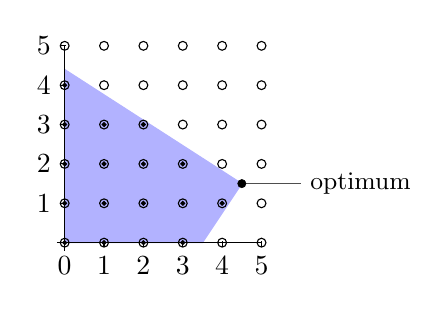
\begin{tikzpicture}[scale=0.5]

  \filldraw[color=blue!30]
  (0,0) -- (3.5,0) -- (4.5,1.5) -- (0,4.4) -- cycle;

  \halfplane{0,0}{5,0}{+}{0.5cm}{0.8cm}
  \halfplane{3.5,0}{4.5,1.5}{+}{0.2cm}{2.4cm}
  \halfplane{0,4.4}{4.5,1.5}{-}{0.5cm}{2.4cm}
  \halfplane{0,0}{0,5}{-}{0.5cm}{1cm}

  %\draw 
  %  (0,3.5) node[anchor=south west]{$x\ge 0$}
  %  (2,3.5) node[anchor=south west]{$x\le 2$}
  %  (2.5,1.8) node[anchor=south west]{$x\ge y$}
  %  (2.5,0.3) node[anchor=south west] {$y\ge 0$};


  \draw
    \foreach \x in {0,...,5}
      \foreach \y in {0,...,5}
      {(\x,\y) circle (3.2pt)};

  \filldraw
  \foreach \x in {0,...,2}
      \foreach \y in {0,...,2}
      {(\x,\y) circle (1.4pt)};
  
  \filldraw   
  \foreach \p in {(0,3),(0,4),(1,3),(3,2),(3,1),(4,1),(2,3),(3,0)}
      {\p circle (1.4pt)};

  %axis
  \draw (-.2,0) -- coordinate (x axis mid) (5,0);
  \draw (0,-.2) -- coordinate (y axis mid) (0,5);
  %ticks
  \foreach \x in {-0,...,5}
      \draw (\x,1pt) -- (\x,-3pt);
  \foreach \x in {0,...,5}
      \draw (\x,-3pt) node[anchor=north] {\x};
  \foreach \y in {1,...,5}
      \draw (1pt,\y) -- (-3pt,\y)
          node[anchor=east] {\y};

  \filldraw[very thin]
    (4.5,1.5) circle (3pt)
    (6,1.5) -- (4.5,1.5)
    (6,1.5) node[anchor=west] {{\small optimum}};

    
\end{tikzpicture}
\mycaption{Prípustné riešenia lineárneho programu a jeho celočíselnej reštrikcie.}
\end{center}

\noindent Na prvý pohľad by sa možno zdalo, že ide iba o kozmetický problém:
nájdeme optimálne riešenie spojitej verzie, vhodne ho zaokrúhlime a dostaneme,
ak nie priamo optimum, tak určite niečo blízke optimu.  Na druhý pohľad začne
byť vidno, že to také jednoduché nebude: ak by nám lineárny program, ktorý
hľadá optimálny spôsob cestovania odporučil kúpiť 0.5 letenky a 0.5 vlakového
lístka, vhodné zaokrúhlenie je vlastne celé riešenie. Ako vidno z nasledujúceho
obrázka, najbližšie celočíselné riešenie môže byť od optimálneho pomerne ďaleko
a nie je zrejmé, ako by sme ho mali hľadať.

\begin{center}
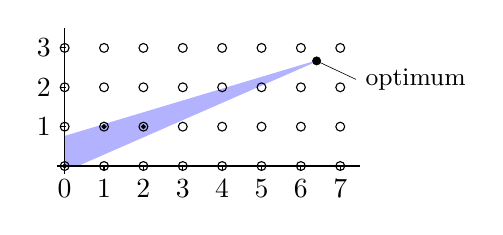
\begin{tikzpicture}[scale=0.5]

  \filldraw[color=blue!30]
  (0,0) -- (0.3,0) -- (6.4,2.67) -- (0,0.75) -- cycle;

  \halfplane{0,0}{7,0}{+}{0.5cm}{0.8cm}
  \halfplane{0.3,0}{6.4,2.67}{+}{0.2cm}{2.4cm}
  \halfplane{0,0.75}{6.4,2.67}{-}{0.5cm}{2.4cm}
  \halfplane{0,0}{0,3}{-}{0.5cm}{1cm}



  \draw
    \foreach \x in {0,...,7}
      \foreach \y in {0,...,3}
      {(\x,\y) circle (3.2pt)};

  \filldraw   
  \foreach \p in {(0,0),(1,1),(2,1)}
      {\p circle (1.4pt)};

  %axis
  \draw (-.2,0) -- coordinate (x axis mid) (7.5,0);
  \draw (0,-.2) -- coordinate (y axis mid) (0,3.5);
  %ticks
  \foreach \x in {-0,...,7}
      \draw (\x,1pt) -- (\x,-3pt);
  \foreach \x in {0,...,7}
      \draw (\x,-3pt) node[anchor=north] {\x};
  \foreach \y in {1,...,3}
      \draw (1pt,\y) -- (-3pt,\y)
          node[anchor=east] {\y};

  \filldraw[very thin]
    (6.4,2.67) circle (3pt)
    (7.4,2.2) -- (6.4,2.67)
    (7.4,2.2) node[anchor=west] {{\small optimum}};

\end{tikzpicture}
\end{center}

\noindent Pridaním dodatočných obmedzení, že niektoré z premenných lineárneho
programu musia byť celočíselné, dostávame tzv. celočíselné lineárne programy:


\begin{framed}
  \begin{dfn}
    {\em Celočíselný lineárny program} (ILP) v normálnom tvare je linárny program
    $$ \max_{\bm{x}\in\R^n}\left\{ \bm{c}\tr\bm{x} \mid A\bm{x}=\bm{b},\;\bm{x}\ge\bm{0}\right\}$$
    s dodatočnými obmedzeniami tvaru $x_i\in\Z$.
  \end{dfn}
\end{framed}

\noindent Skúseného čitateľa isto neprekvapí, že celočíselné obmedzenia
podstatne zvyšujú vyjadrovaciu schopnosť lineárnych programov. Pri formulovaní
zložitejších vzťahov pomocou ILP hrajú dôležitú úlohu tzv. {\em indikátorové
premenné}: sada premenných $\delta_1,\ldots,\delta_k\in\Z$ s obmedzeniami
\begin{align*}
  \delta_1+\delta_2+\cdots+\delta_k&=1\\
  \delta_i&\ge0\text{\ pre\ }i=1\ldots k
\end{align*}
má tú vlastnosť, že v ľubovoľnom prípustnom riešení je práve jedna $\delta_i=1$
a ostatné sú nulové.  Indikátorové premenné umožňujú vyjadriť alternatívu medzi
viacerými možnosťami a tým napríklad popísať zložité nekonvexné obory hodnôt.
Ako demonštráciu predpokladajme, že chceme maximalizovať funkciu $f(x,y)=x+y$
na takejto množine \dom:

\begin{myfig}{0.4\textwidth}{svg/nekonvex-a}
\end{myfig}

\noindent
Množinu \dom môžme rozdeliť na 5 častí
\begin{myfig}{0.4\textwidth}{svg/nekonvex}
\end{myfig}
z ktorých každú vieme reprezentovať lineárnymi obmedzeniami:
\begin{align*}
  x&\ge0    & x&\ge1 & x&\ge1 & x&\ge2    & x&\ge4\\
  x&\le1    & x&\le2 & x&\le2 & x&\le3    & x&\le5\\
  y&\ge1-x  & y&\ge2 & y&\ge0 & y&\ge x-2 & y&\le6x-24\\
  y&\le2+x  & y&\le3 & y&\le1 & y&\le5-x  & y&\le-6x+30\\
   &        &  &     &  &     &  &        & y&\ge0
\end{align*}
Zavedieme indikátorové premenné $\delta_1,\ldots,\delta_5\in\Z$ a každú sadu
obmedzení určujúcich jednu oblasť prepíšeme tak, aby v prípade, že príslušný
indikátor je nulový, dávali triviálne obmedzenia a aby sa zachovali pôvodné
obmedzenia, ak je indikátor jednotkový. Dostaneme tak ILP: maximalizovať $x+y$
pri obmedzeniach

\begin{align*}
  x&\ge0                  & x&\ge\delta_2    & x&\ge\delta_3    & x&\ge2\delta_4            & x&\ge4\delta_5\\
  x&\le5-4\delta_1        & x&\le5-3\delta_2 & x&\le5-3\delta_3 & x&\le5-2\delta_4          & x&\le5\\
  y&\ge\delta_1-x         & y&\ge2\delta_2   & y&\ge0           & y&\ge-5+3\delta_4+x  & y&\le3-27\delta_5+6x\\
  y&\le3-\delta_1+x   & y&\le3           & y&\le3-4\delta_3 & y&\le8-3\delta_4-x    & y&\le33-3\delta_5-6x\\
   &                      &  &               &  &               &  &                        & y&\ge0
\end{align*}
\begin{align*}
  \delta_1+\delta_2+\delta_3+\delta_4+\delta_5&=1\\
  \delta_i&\ge0, \delta_i\in\Z\text{\ pre\ }i=1\ldots 5
\end{align*}

\noindent Inou v praxi dôležitou vlastnosťou celočíselných lineárnych programov
je schopnosť optimalizovať nelineárne účelové funkcie.  Predpokladajme, že v
predchádzajúcom príklade namiesto funkcie $f(x,y)=x+y$ chceme maximalizovať
funkciu $f(x,y)=\varphi(x+y)$, kde funkcia $\varphi$ je zložená z lineárnych
úsekov:
\begin{myfig}{0.55\textwidth}{svg/nonlinear-a}
\end{myfig}

\noindent Zavedieme štyri pomocné premenné $z_1,z_2,z_2,z_3,z_4$, ktoré
udávajú, aká časť príslušného intervalu je ``zaplnená'' hodnotou $x+y$:
$$x+y=z_1+z_2+z_3+z_4$$

\noindent
\begin{minipage}[t]{0.5\textwidth}
  \vskip 0pt
\begin{myfig}{\textwidth}{svg/nonlinear}
\end{myfig}
\end{minipage}
\hspace*{1cm}
\begin{minipage}[t]{0.5\textwidth-1cm}
\vskip 0pt
Potrebujeme pridať ďalšie obmedzenia, ktoré zabezpečia, že $z_i$ sa budú
``zapĺňať postupne'', t.j. ak $z_i$ je nenulová, tak $z_{i-1}$ je na svojej
maximálnej hodnote.  Pridáme tri binárne premenné $\alpha_1,\alpha_2,\alpha_3$,
kde $\alpha_i\in\Z$, $0\le\alpha_i\le1$, pričom chceme, aby premenná
$\alpha_i\in\{0,1\}$ udávala, či je $z_{i+1}$ nenulová. Obmedzenia
\begin{align*}
  2\alpha_1&\le z_1\le2\\
  \alpha_2&\le z_2\le\alpha_1\\
  2\alpha_3&\le z_3\le2\alpha_2\\
  0&\le z_4\le3\alpha_3
\end{align*}
vynútia požadované vlastnosti: napríklad ak $\alpha_1=0$, tak $0\le z_1\le2$, ale $z_2=z_3=z_4=0$. Ak ale $\alpha_1=1$, $z_1=2$ a $\alpha_2\le z_2\le1$.
S takto nastavenými premenným $z_1,\ldots,z_4$ ľahko vyjadríme účelovú funkciu
\end{minipage}

$$f(x,y,z_1,\ldots,z_4,\alpha_1,\ldots,\alpha_3,\delta_1,\ldots,\delta_5)=1+\frac{1}{2}z_1+4z_2-2z_3-\frac{1}{2}z_4$$


\vskip 1ex \noindent Prezentované príklady snáď utvrdili čitateľovu intuíciu,
že pomocou ILP sa dajú zapísať oveľa zložitejšie problémy, ako pomocou
lineárnych programov, a teda aj riešenie ILP by malo byť oveľa ťažšie. Ukážeme
si, že tomu tak naozaj je: už aj úloha zistiť, či daný ILP má vôbec nejaké
prípustné riešenie, je \NP-úplná, a teda neočakávame, že by sme našli
polynomiálny algoritmus na riešenie ILP. Pre úplnosť zopakujeme definíciu
problému  \sat

\begin{framed}
  \begin{dfn}
    \label{dfn:sat}
    Majme $n$ logických premenných $x_1,\ldots,x_n\in\{true,false\}$. {\em
    Literál} je premenná $x_i$ alebo jej negácia $\neg{x_i}$. {\em Klauzula} je
    dizjunkcia literálov $C=l_1\vee l_2\vee\cdots\vee l_{k_C}$.  Formula v {\em
    konjunktívnej normálne forme} (CNF) je konjunkcia klauzúl $F=C_1\wedge
    C_2\wedge\cdots\wedge C_m$. Problém \sat je rozhodovací problém, v ktorom
    je na vstupe daná formula $F$  v CNF a úlohou je zistiť, či existuje
    ohodnotenie premenných $x_1,\ldots,x_n$ tak, aby $F$ bola splnená.
  \end{dfn}
\end{framed}

\noindent Základné tvrdenie z teórie je Cook-Lewinova veta, ktorá hovorí, že
problém \sat je \NP-úplný, t.j. keby existoval polynomiálny algoritmus pre
\sat, platilo by $\P=\NP$.  Teraz ukážeme, že keby existoval polynomiálny
algoritmus \algA, ktorý pre daný ILP zistí, či má nejaké prípustné riešenie,
existoval by aj polynomiálny algoritmus \algA' riešiaci \sat.  Predpokladajme,
že máme algoritmus \algA a ideme popísať, ako pracuje \algA'.  Nech vstupná
formula $F$ pozostáva z klauzúl $C_1,\ldots,C_m$. Označme $P_i$ množinu
premenných, ktoré sa vyskytujú v $C_i$ ako pozitívne literály, a $N_i$ množinu
tých premenných, ktoré sa v $C_i$ vyskytujú v negovaných literáloch. Napríklad
pre klauzulu $C_i=(x_1\vee\neg{x_2}\vee x_3)$ je $P_i=\{x_1,x_3\}$ a
$N_i=\{x_2\}$.  Zostrojíme zadanie ILP $I$ tak, že každej logickej premennej
$x_i$ zo vstupnej formuly bude prirodzeným spôsobom zodpovedať (rovnako
nazvaná) premenná $x_i\in\Z$ s obmedzeniami $0\le x_i\le1$.  Splňujúce
ohodnotenie musí spĺňať aspoň jeden literál v každej klauzule $C_i$, čo sa dá
vyjadriť obmedzením
$$\sum_{x\in P_i}x + \sum_{x\in N_i}(1-x) \ge 1$$
Napríklad pre formulu
$$(x_1\vee x_2\vee x_3)\wedge(\neg{x_1}\vee\neg{x_2}\vee\neg{x_3})\wedge(x_1\vee\neg{x_2}\vee\neg{x_3})\wedge(\neg{x_1}\vee\neg{x_2}\vee x_3)\wedge(\neg{x_1}\vee x_2\vee x_3)$$
dostaneme obmedzenia
\begin{align*}
  x_1+x_2+x_3&\ge1\\
  (1-x_1)+(1-x_2)+(1-x_3)&\ge1\\
  x_1+(1-x_2)+(1-x_3)&\ge1\\
  (1-x_1)+(1-x_2)+x_3&\ge1\\
  (1-x_1)+x_2+x_3&\ge1\\
  x_1,x_2,x_3&\ge0\\
  x_1,x_2,x_3&\le1
\end{align*}
Zjavne každé splňujúce ohodnotenie $F$ je prípustným riešením $I$ a naopak.
Preto $F$ je splniteľná práve vtedy, ak existuje prípustné riešenie $I$.

\begin{prob}
  Skúste iné známe \NP-ťažké problémy (napr. problém obchodného cestujúceho, nájdenie najväčšej kliky v grafe, \ldots) redukovať na ILP.
\end{prob}

\vskip 1ex \noindent Naše predchádzajúce úvahy môžme zhrnúť takto: ILP je
všeobecný formalizmus, pomocou ktorého sa dajú zapísať mnohé optimalizačné
problémy. Táto výrazová sila je zároveň jeho slabinou, lebo neočakávame, že by
existoval efektívny algoritmus, ako ILP riešiť.

\subsection*{Dobrý: \maxWBmatching}

Predpokladajme, že máme za úlohu napísať  program, ktorý hrá strategickú hru. V
jednom ťahu má k dispozícii niekoľko figúr, z ktorých každá môže potenciálne
zaútočiť na niektorú nepriateľskú figúru (najprv sa musí presunúť na niektoré
priľahlé políčko, pričom sa dve figúry nemôžu presunúť na to isté políčko).
Každý potenciálny útok má číselne vyjadrenú silu a cieľom je presunúť figúry
tak, aby celková sila útoku bola čo najväčšia. 

\begin{myfig}{0.8\textwidth}{svg/match}
  Každá z figúr v spodnom riadku sa môže presunúť na niektoré z vyznačených
  modrých políčok a zaútočiť na nepriateľskú figúru; čísla udávajú silu útoku.
  Najsilnejší útok je zvýraznený.
\end{myfig}


\noindent
Problém, ktorý riešime, je známy ako problém najväčšieho bipartitného párovania\footnote{Tento problém je trochu výnimka: väčšina problémov 
  prezentovaných v tomto kurze sú \NP-ťažké, ale \maxWBmatching nie. Čitateľ možno pozná
efektívny algoritmus na riešenie tohoto problému, napriek tomu ho poprosíme, aby sledoval náš prístup z didaktivkých dôvodov.}:

\begin{framed}
  \begin{dfn}
    \label{dfn:maxWBmatching}
    Majme daný bipartitný graf s hranami ohodnotenými nezápornými reálnymi
    číslami. Cieľom problému \maxWBmatching je nájsť množinu hrán s najväčším
    súčtom váh tak, aby žiadne dve vybraté hrany nezdieľali vrchol.
  \end{dfn}
\end{framed}

\noindent Problém \maxWBmatching sa ľahko zapíše ako ILP. Nech je na vstupe
bipartitný graf $G=(V,E)$ s ohodnotením $\omega:E\mapsto\R^+$.  Pre každú hranu
$e\in E$ budeme mať premennú $x_e\in\{0,1\}$, ktorá bude určovať, či je daná
hrana vybratá. Cieľom je maximalizovať súčet váh vybratých hrán, t.j.
$\max\sum_{e\in E}\omega_ex_e$. Obmedzenia musia zabezpečiť, aby z okolia
každého vrchola $v$ bola vybratá najviac jedna hrana. Celý ILP potom vyzerá
takto (obmedzenia $x_e\le1$ netreba písať explicitne, nakoľko vyplývajú z
ostatných):

\begin{equation}
\label{eq:ILPa:1}
\begin{array}{rrcll}
  {\rm maximalizovať}     & \multicolumn{1}{l}{\sum\limits_{e\in E}\omega_ex_e}\\[3ex]
  {\rm pri\ obmedzeniach} & \sum\limits_{e\in E\atop e=(v,w)}x_e&\le&1& \;\;\;\forall v\in V\\
                          & x_e&\ge&0& \;\;\;\forall e\in E\\
                          & x_e&\in&\Z
\end{array}
\end{equation}

\noindent
Napríklad pre graf vľavo dostaneme obmedzenia\\
\begin{minipage}[t]{0.4\textwidth}
  \vskip 0pt
  \begin{myfig}{0.8\textwidth}{svg/match-2}
\end{myfig}
\end{minipage}
\begin{minipage}[t]{0.6\textwidth}
\vskip 0pt
\begin{align}
  x_{e_1}&\le1\notag\\
  x_{e_2}+x_{e_4}&\le1\notag\\
  x_{e_3}+x_{e_5}&\le1\notag\\
  x_{e_1}+x_{e_2}+x_{e_3}&\le1\label{eq:ILPa:2}\\
  x_{e_4}+x_{e_5}&\le1\notag\\
  x_{e_1},x_{e_2},x_{e_3},x_{e_4},x_{e_5}&\ge0\notag
  %x_{e_1},x_{e_2},\ldots,x_{e_5}&\in\Z\\
\end{align}
\end{minipage}

\noindent Keďže na riešenie ILP nemáme efektívny algoritmus, môžme skúsiť
vyriešiť {\em\bfseries relaxovaný} LP, kde z programu (\ref{eq:ILPa:1})
vynecháme obmedzenia $x_e\in\Z$.  Zjavne, všetky prípustné riešenia ILP sú aj
prípustnými riešeniami relaxovaného programu, preto optimum relaxovaného
programu je horný odhad optimálneho riešenia ILP.  Ako sme však videli, riešiť
relaxovaný program vo všeobecnosti  nie je dobrý nápad, lebo optimálne riešenie
relaxovaného problému môže byť  od optimálneho riešenia pôvodného ILP veľmi
ďaleko.  Lenže my sa teraz nezaoberáme všeobecným ILP, ale konkrétne takým,
ktoré sme dostali uvedeným postupom z nejakého bipartitného grafu.  Môžme teda
dúfať, že dodatočná štruktúra obmedzení spôsobí, že riešenie relaxovaného
problému bude niesť nejakú informáciu o pôvodnom ILP.  
Skúsme napríklad 
pre obmedzenia z (\ref{eq:ILPa:2}) nastaviť $\omega_{e_1}=1$ a
$\omega_{e_2}=\cdots=\omega_{e_5}=10$ a vyriešiť relaxovaný program.
Ak spustíme simplexový algoritmus\footnote{Pre väčší dramatický efekt to odporúčame čitateľovi naozaj
vyskúšať.}, na naše potešenie bude nájdené optimálne riešenie celočíselné, aj
keď existujú aj neceločíselné optimálne riešenia  (napr. $x_{e_1}=0$,
$x_{e_2}=\cdots=x_{e_5}=\frac{1}{2}$).  Môžme to skúsiť s inými váhami aj na
iných grafoch a výsledky budú rovnaké: simplexový algoritmus vždy nájde
celočíselné optimálne riešenie relaxovaného programu, ktoré je na základe
predchádzajúcich úvah optimálnym riešením ILP.
Skúsme teraz zistiť príčinu tohto správania.
Napíšme si náš program v maticovom tvare
$$\max\{\bm{c}\tr\bm{x}\mid A\bm{x}\le\bm{b},\;\bm{x}\ge\bm{0}\}$$
kde
\begin{align*}
\bm{c}&=\left(\begin{array}{c}1\\10\\10\\10\\10\end{array}\right)&
A&=\left(\begin{array}{ccccc}1&0&0&0&0\\0&1&0&1&0\\0&0&1&0&1\\1&1&1&0&0\\0&0&0&1&1\end{array}\right)&
\bm{x}&=\left(\begin{array}{c}x_{e_1}\\x_{e_2}\\x_{e_3}\\x_{e_4}\\x_{e_5}\end{array}\right)&
\bm{b}&=\left(\begin{array}{c}1\\1\\1\\1\\1\end{array}\right)
\end{align*}
Matica $A$ je tzv. {\em
matica incidencie} bipartitného grafu, t.j. matica, ktorá má riadok pre každý
vrchol a stĺpec pre každú hranu, pričom v každom stĺpci sú práve dve jednotky,
a to práve v riadkoch prislúchajúcich koncovým vrcholom danej hrany.
Zároveň vidíme, že  podmienka $x_{e_1}\le1$
vyplýva z nezápornosti a podmienky $x_{e_1}+x_{e_2}+x_{e_3}\le1$, a tak prvý riadok môžeme vynechať.
Pridáme rezervné premenné a dostaneme program v normálnom tvare:
\begin{equation}
  \label{eq:ILPa:3}
  \max\{\bm{\tilde{c}}\tr\bm{\tilde{x}}\mid \tilde{A}\bm{\tilde{x}}=\bm{\tilde{b}},\;\bm{\tilde{x}}\ge\bm{0}\}
\end{equation}
kde
\begin{align*}
\bm{\tilde{c}}&=\left(\begin{array}{c}1\\10\\10\\10\\10\\0\\0\\0\\0\end{array}\right)&
\tilde{A}&=\left(\begin{array}{ccccccccc}0&1&0&1&0&1&0&0&0\\0&0&1&0&1&0&1&0&0\\1&1&1&0&0&0&0&1&0\\0&0&0&1&1&0&0&0&1\end{array}\right)&
\bm{\tilde{x}}&=\left(\begin{array}{c}x_{e_1}\\x_{e_2}\\x_{e_3}\\x_{e_4}\\x_{e_5}\\s_1\\s_2\\s_3\\s_4\end{array}\right)&
\bm{\tilde{b}}&=\left(\begin{array}{c}1\\1\\1\\1\end{array}\right)
\end{align*}

\noindent
Pre každú bázu $B$, je matica $\tilde{A}_B$ regulárna štvorcová matica $4\times 4$ a nenulové premenné príslušného bázového riešenia sú riešením
systému
$$\tilde{A}_B\bm{\tilde{x}}_B=\bm{\tilde{b}},$$
takže podľa Cramerovho pravidla je $i$-ta zložka riešenia
$$\frac{\det\left(\tilde{A}_B\langle i\rangle\right)}{\det\left(\tilde{A}_B\right)}$$
kde $\tilde{A}_B\langle i\rangle$ je matica, ktorú dostaneme z $\tilde{A}_B$, ak $i$-ty stĺpec nahradíme vektorom $\bm{\tilde{b}}$.
Napríklad pre bázu $B=(2,4,7,8)$ dostávame systém
$$\tilde{A}_B\bm{\tilde{x}}_B=\left(\begin{array}{cccc}1&1&0&0\\0&0&1&0\\1&0&0&1\\0&1&0&0\end{array}\right)
\left(\begin{array}{c}x_{e_2}\\x_{e_4}\\s_2\\s_3\end{array}\right)=
\left(\begin{array}{c}1\\1\\1\\1\end{array}\right)
$$
Pri použití Cramerovho pravidla potrebujeme tieto determinanty:
$$\det\left(\tilde{A}_B\right)=\left|\begin{array}{cccc}1&1&0&0\\0&0&1&0\\1&0&0&1\\0&1&0&0\end{array}\right|=1$$
\renewcommand{\tmp}{\bm{{\color{red}1}}}
\begin{align*}
\left|\begin{array}{cccc}\tmp&1&0&0\\\tmp&0&1&0\\\tmp&0&0&1\\\tmp&1&0&0\end{array}\right|&=0&
\left|\begin{array}{cccc}1&\tmp&0&0\\0&\tmp&1&0\\1&\tmp&0&1\\0&\tmp&0&0\end{array}\right|&=1&
\left|\begin{array}{cccc}1&1&\tmp&0\\0&0&\tmp&0\\1&0&\tmp&1\\0&1&\tmp&0\end{array}\right|&=1&
\left|\begin{array}{cccc}1&1&0&\tmp\\0&0&1&\tmp\\1&0&0&\tmp\\0&1&0&\tmp\end{array}\right|&=1
\end{align*}
Dostali sme riešenie
  $x_{e_2}=0, x_{e_4}=1, s_2=1, s_4=1$
čo zodpovedá (neoptimálnemu) celočíselnému riešeniu, v ktorom je vybratá iba hrana $e_4$.
Rezervné premenné $s_2=s_3=1$ hovoria, že vrcholy $v_3$ a $v_4$ (druhý a tretí riadok matice $\tilde{A}$) majú voľnú kapacitu.
Namiesto toho, aby sme takýmto spôsobom overili všetkých ${9\choose4}=126$ potenciálnych báz, pokúsime sa tento postup zovšeobecniť.

\begin{framed}
  \begin{dfn}
    Štvorcová matica $A$ s celočíselnými prvkami sa nazýva {\em unimodulárna}, ak $det(A)=\pm1$, kde $det$ označuje determinant matice.
    
    Matica (nie nutne štvorcová) $A$ s celočíselnými prvkami sa nazýva {\em totálne unimodulárna} (TUM), ak každá jej regulárna 
    štvorcová podmatica (t.j. matica rozmerov $k\times k$, ktorá vznikne a $A$ výberom nejakých $k$ riadkov a nejakých $k$ stĺpcov)
    je unimodulárna
  \end{dfn}
\end{framed}

\noindent
Táto definícia špeciálne znamená, že všetky prvky TUM matice $A$ sú $0,\pm1$: každý prvok je totiž podmatica rozmerov $1\times1$.

\begin{veta}
  \label{thm:tumInteger}
  Majme lineárny program v normálnom tvare 
  $\max\{\bm{c}\tr\bm{x}\mid A\bm{x}=\bm{b},\;\bm{x}\ge\bm{0}\},$
  kde $A$ je TUM matica a \bm{b} je coločíselný vektor. 
  Potom všetky bázové riešenia sú celočíselné.
\end{veta}
\begin{dokaz}
  Uvažujme bázu $B$. $A_B$ je štvorcová regulárna matica a nenulové zložky bázového riešenia sú riešenia systému
  $A_B\bm{x}_B=\bm{b}$ a dajú sa explicitne vyjadriť ako
  $$\frac{\det\left(A_B\langle i\rangle\right)}{\det(A_B)}.$$
  Keďže $A$ je TUM, $\det(A_B)=\pm1$. Pre výpočet determinantu $\det\left(A_B\langle i\rangle\right)$ použijeme jeho rozvoj
  podľa $i$-teho stĺpca
  $$\det\left(A_B\langle i\rangle\right)=(-1)^{i+1}b_1C_1+\cdots+(-1)^{i+m}b_mC_m,$$
  kde $C_j$ sú determinanty štvorcových podmatíc $A$, a teda $C_j\in\{0,\pm1\}$. Keďže podľa predpokladu $b\in\Z$, dôkaz je hotový.
\end{dokaz}

\noindent
V skutočnosti sme použili iba slabšiu vlastnosť ako unimodularita: stačilo nám aby determinant regulárnej podmatice $m\times m$ bol $\pm1$ a
ostatné determinanty štvorcových podmatíc boli celočíselné. Ničmenej trieda problémov s TUM maticami je dostatočne bohatá. Ukážeme teraz niekoľko
tvrdení o TUM:

\begin{veta}
  \label{thm:idTum}
  Nech $A$ je TUM rozmerov $n\times m$ a nech $k\le m$. Potom
$B:=\left(\begin{array}{c|c}\multirow{2}{*}{{\Large A}}&0\\\cline{2-2} &I_k\end{array}\right)$, kde
  $I_k$ je identická matica rozmerov $k\times k$, je TUM.
\end{veta}
\begin{dokaz}
  Nech $C$ je ľubovoľná regulárna štvorcová podmatica matice $B$, t.j. $C=(C_1\mid C_2)$, kde
  $C_1$ sú stĺpce matice $A$ a $C_2$ sú stĺpce z $I$. Riadky $C$ preusporiadame tak, že
  riadky, ktoré sú nulové v $C_2$ dáme na vrch, a teda 
$$C=\left(\begin{array}{c|c}A'&0\\\hline X&I_\ell\end{array}\right)$$
  kde $A'$ je štvorcová podmatica $A$. Keďže $C$ je regulárna, platí $\det(C)=\pm1$.
\end{dokaz}

\begin{veta}
  Majme lineárny program v tvare
  $\max\{\bm{c}\tr\bm{x}\mid A\bm{x}\le\bm{b},\;\bm{x}\ge\bm{0}\},$
  kde $A$ je TUM matica a \bm{b} je coločíselný vektor.
  Potom všetky bázové riešenia sú celočíselné.
\end{veta}
\begin{dokaz}
  Podľa Vety~\ref{thm:idTum} je 
   matica $(A\mid I)$, kde $I$ je identická matica $m\times m$, TUM; tvrdenie  vyplýva z 
  postupu normalizácie lineárnych programov (matica $I$ zodpovedá rezervným premenným).
\end{dokaz}

\begin{veta}
  \label{thm:unimod}
  Nech $A$ je matica s prvkami $a_{ij}\in\{0,\pm1\}$, ktorej riadky sa dajú rozdeliť na dve množiny $I_1$, $I_2$ tak, že
  \begin{enumerate}
    \item Ak má nejaký stĺpec dva prvky s rovnakým znamienkom, ich príslušné riadky sú v rôznych množinách
    \item Ak má nejaký stĺpec dva prvky s rôznym znamienkom, ich príslušné riadky sú v rovnakej množine.
  \end{enumerate}
  Potom $A$ je TUM.
\end{veta}

\begin{dokaz}
  Potrebujeme dokázať, že každá regulárna štvorcová podmatica $k\times k$ má determinant $\pm1$. Toto tvrdenie
  dokážeme indukciou na veľkosť podmatíc. Bázu indukcie tvoria podmatice $1\times 1$, t.j. prvky matice.
  Predpokladajme teraz, že tvrdenie platí pre podmatice rozmerov $k-1\times k-1$. Zoberme si ľubovoľnú štvorcovú
  podmaticu $C$ rozmerov $k\times k$. Ak $C$ má všetky stĺpce nulové, je singulárna. Ak má nejaký stĺpec s práve jedným
  nenulovým prvkom (t.j. $\pm1$), použijeme rozvoj determinantu podľa tohto stĺpca a z indukčného predpokladu
  dostaneme $\det(C)=\pm1$. Nech teda každý stĺpec $C$ má aspoň dva nenulové prvky. Z podmienok vety ale vyplýva,
  že pre každý stĺpec $j$ platí 
  $$\sum\limits_{i\in I_1}c_{ij}=\sum\limits_{i\in I_2}c_{ij}$$
  Preto lineárna kombinácia riadkov je $0$ a $\det(C)=0$.
\end{dokaz}

\begin{dosl}
  Každý lineárny program tvaru $$\max\{\bm{c}\tr\bm{x}\mid A\bm{x}\le\bm{b},\;\bm{x}\ge\bm{0}\}$$ alebo
  $$\max\{\bm{c}\tr\bm{x}\mid A\bm{x}\le\bm{b},\;\bm{x}\ge\bm{0}\},$$ kde \bm{b} je celočíselný vektor a $A$ je
   \begin{enumerate}
     \item matica incidencie neorientovaného bipartitného grafu, alebo
     \item matica incidencie orientovaného grafu\footnote{matica, ktorá má riadok pre každý vrchol a stĺpec pre každú orientovanú hranu, pričom v stĺpci prislúchajúcom hrane $(v_i,v_j)$ je
       na $i$-tom riadku 1, a na $j$-tom riadku -1 (ostatné prvky sú nulové).}
   \end{enumerate}
   má všetky bázové riešenia celočíselné.
\end{dosl}
\begin{dokaz}
  V prípade 1) označme $I_1$ riadky prislúchajúce vrcholom jednej bipartície, 
  v prípade 2) budú v $I_1$ všetky riadky. Použijeme vetu~\ref{thm:unimod}.
\end{dokaz}

\noindent
Teraz vidíme, že problém \maxWBmatching je iba jedným z neveľkej triedy problémov, kde simplexový algoritmus na relaxovanom
lineárnom programe vždy nájde celočíselné optimum. Pochopiteľne, pri \NP-ťažkých problémoch už také šťastie 
nebudeme mať. Napriek tomu, niekedy relaxovaný lineárny program pomôže nájsť aspoň približné riešenie, ako
uvidíme v ďalších častiach.

\begin{prob}
  Zapíšte problém hľadania najkratšej cesty ako lineárny program.
\end{prob}

%%%%%%%%%%%%%%%%%%%%%%%%%%%%%%%%%%%%%%%%%%%%%%%%%%%%%%%%%%%%%%%%%%%%%%%%%%%%%%%%%%%%%%%%%%%%%%%%%%%%%%%%%%%%%%
\subsection*{Zlý: \minvcover}

Problémy, v ktorých relaxovaný lineárny program nájde optimálne riešenie, sú skôr výnimkou. Aj v iných prípadoch
však môže riešenie relaxovaného problému pomôcť. Ako príklad použijeme aplikáciu z výpočtovej biológie
(viď. \cite{lBILS01}). Jedince jedného druhu majú veľmi podobný genóm, ktorý sa líši iba na niekoľkých
miestach. Cieľom je identifikovať tzv. {\em snipy} ({\em Single Nucleotide Polymorhism}) v genóme,
čo sú miesta v genóme, kde sa môžu vyskytovať rôzne hodnoty, pričom naokolo je rovnaký obsah. 
Genóm je sada sekvencovaných fragmentov a vstupom je matica, ktorá udáva hodnotu ($A$, $B$ alebo $-$ pre neurčené) 
daného
snipu na danom fragmente. Cieľom je nájsť ofarbenie fragmentov dvoma farbami tak, aby zodpovedali 
dvom alternatívnym genómom.

\begin{myfig}{0.4\textwidth}{svg/SNP}
Konfigurácia fragmentov $f_4$,$f_5$ a snipov  $s_2$,$s_3$ tvorí  konflikt: 
podľa snipu $s_2$ musia fragmenty $f_4$ a $f_5$
mať rôzne farby, podľa snipu $s_3$ potom ale všetky hodnoty $s_3$ musia byť $B$, čiže $s_3$ nie je snip.
Keby hodnota $s_3$ na fragmente $f_6$ bola $A$, zelené a červené fragmenty by zodpovedali dvom 
alternatívnym genómom.
\end{myfig}

\noindent
Vstupné dáta vždy obsahujú chyby. Konfigurácia dvoch fragmentov a dvoch snipov ako na predchádzajúcom 
obrázku tvorí konflikt: jeden zo snipov musel byť prečítaný zle a treba ho ignorovať. 
Ak máme pre každý snip číselne vyjadrenú jeho významnosť, môžme zostrojiť konfliktový graf snipov, t.j.
graf, kde snipy sú vrcholy a dva snipy, ktoré sú v konflikte sú spojené hranou. Prvým krokom 
k nájdeniu alternatívnych genómov je vyhodiť
čo možno najmenej snipov tak, aby vo výsledku neboli konflikty. Prirodzene tak dostávame inštanciu
problému \minvcover:

\begin{framed}
  \begin{dfn}
    \label{dfn:minvcover}
Daný je jednoduchý graf $G=(V,E)$ s
vrcholmi ohodnotenými nezápornými váhami, t.j. funkciou $\omega:V\mapsto\R^+$.
Cieľom problému \minvcover je vybrať množinu vrcholov tak, aby každá hrana bola incidentná aspoň s
jedným vybratým vrcholom a celková váha vybratých vrcholov bola minimálna. 
\end{dfn}
\end{framed}



\begin{myfig}{0.8\textwidth}{svg/vertexcover}
  Príklad vrcholového pokrytia. Modré vrcholy majú váhu 1, žlté váhu 2 a červené váhu 13. 
  Celé pokrytie má váhu 47. Dá sa nájsť pokrytie s menšou váhou?
\end{myfig}

\noindent Úloha sa dá jednoducho zapísať ako celočíselný lineárny program. Pre
každý vrchol $v\in V$ zavedieme premennú $x_v\in\{0,1\}$, ktorá indikuje, či je
daný vrchol vybratý.  Celý lineárny program potom vyzerá nasledovne:

\begin{equation}
\label{eq:ILP:1}
\begin{array}{rrcll}
  {\rm minimalizovať}     & \multicolumn{1}{l}{\sum\limits_{v\in V}\omega_vx_v}\\
  {\rm pri\ obmedzeniach} & x_u + x_v&\ge&1& \;\;\;\forall e=(u,v)\in E\\
                          & x_v&\ge&0& \;\;\;\forall v\in V\\
                          & x_v&\in&\Z
\end{array}
\end{equation}

\noindent
Účelová funkcia hovorí, že sa snažíme minimalizovať súčet váh vybraných
vrcholov.  Pre každú hranu $(u,v)\in E$ máme obmedzenie tvaru $x_u+x_v\ge 1$,
ktoré zaručí, že aspoň jeden z koncových vrcholov hrany je vybratý. Obmedzenia
$x_v\ge0$ a $x_v\in\Z$ spolu zaručia $x_v\in\{0,1\}$: ak je v nejakom
prípustnom riešení niektorá hodnota $x_v>1$, nastavením $x_v=1$ ostanú všetky
obmedzenia splnené a, keďže váhy sú nezáporné, hodnota účelovej funkcie sa
nezväčší.

Problém \minvcover je \NP-ťažký, a tak neočakávame, že by sme program
(\ref{eq:ILP:1}) vedeli riešiť v polynomiálnom čase. Uspokojíme sa preto s
aproximáciou: chceme nájsť riešenie, ktorého váha nikdy nie je väčšia ako
dvojnásobok váhy optimálneho riešenia. Takýto algoritmus sa označuje ako
2-aproximačný (v nasledujúcej definícii $r$ nemusí byť konštanta, preto
potrebujeme brať suprémum cez všetky vstupy danej veľkosti):

\begin{framed}
  \begin{dfn}
    Majme optimalizačný problém ${\cal P}$ a polynomiálny algoritmus ${\cal A}$, ktorý ho rieši. 
    Nech $m^\star(\bm{x})$ je hodnota optimálneho riešenia pre vstup \bm{x} a
    $m_{\cal A}(\bm{x})$ je hodnota, ktorú vráti algoritmus $\cal A$. {\em Aproximačný
    pomer algoritmu $\cal A$ na vstupe \bm{x}}je
    $$R_{\cal A}(\bm{x})=\left\{\begin{array}{ll}
        \frac{m^\star(\bm{x})}{m_{\cal A}(\bm{x})}&\text{\ ak $\cal P$ je maximalizačný}\\[3ex]
      \frac{m_{\cal A}(\bm{x})}{m^\star(\bm{x})}&\text{\ ak $\cal P$ je minimalizačný}\end{array}\right.$$
    
  \noindent  
   Algoritmus $\cal A$ je {\em $r(n)$-aproximačný}, ak 
  $$\forall n:\;\sup_{|\bm{x}|=n}R_{\cal A}(\bm{x})\le r(n)$$
 pričom suprémum sa berie cez všetky vstupy dĺžky $n$.

  \end{dfn}
\end{framed}



Začneme tým, že z programu (\ref{eq:ILP:1}) odstránime obmedzenia $x_v\in\Z$, čím
dostaneme relaxovaný lineárny program
\begin{equation}
\label{eq:ILP:2}
\begin{array}{rrcll}
  {\rm minimalizovať}     & \multicolumn{1}{l}{\sum\limits_{v\in V}\omega_vx_v}\\
  {\rm pri\ obmedzeniach} & x_u + x_v&\ge&1& \;\;\;\forall e=(u,v)\in E\\
                          & x_v&\ge&0& \;\;\;\forall v\in V\\
\end{array}
\end{equation}
ktorý vieme efektívne vyriešiť. Nech teraz \opt je optimálne (celočíselné)
riešenie programu (\ref{eq:ILP:1}) a \bm{x} je optimálne riešenie programu
(\ref{eq:ILP:2}).  Zjavne $\bm{\omega}\tr\bm{x}\le\opt$ (relaxáciou sme množinu
prípustných riešení iba zväčšili, preto optimum sa mohlo iba zmenšiť). Otázka,
ktorá nás trápi, je, ako ďaleko je \opt od  $\bm{\omega}\tr\bm{x}$ a ako dostať
z \bm{x} celočíselné riešenie, ktoré nebude ďaleko od \opt.  V tomto prípade sa
ukáže, že máme šťastie a $\opt\le2\bm{\omega}\tr\bm{x}$.  Situácia je ako na
nasledujúcom obrázku:

\begin{myfig}{0.7\textwidth}{svg/vcoverrelax}
\end{myfig}

\noindent Spomedzi možných hodnôt účelovej funkcie je $\bm{\omega}\tr\bm{x}$
minimálna. Nás zaujíma \opt, čo je minimálne celočíselné riešenie. Ak sa nám
podarí skonštruovať celočíselné riešenie s váhou nanajvýš
$2\bm{\omega}\tr\bm{x}$, máme zaručené, že jeho váha je najviac $2\opt$.

\noindent Najjednoduchší spôsob, ako z \bm{x} dostať celočíselné riešenie je
zaokrúhliť hodnoty $x_v$. Vieme, že všetky $x_v\ge 0$ a takisto bez ujmy na
všeobecnosti $x_v\le 1$ (v optimálnom riešení nemá zmysel mať hodnotu $x_v>1$:
keby to tak bolo, nastavením $x_v=1$ sa hodnota $\omega_vx_v$ nezväčší a
všetky obmedzenia ostanú splnené), preto zaokrúhlenie vlastne znamená vybrať
tie vrcholy, pre ktoré $x_v\ge\frac{1}{2}$.  Najprv si treba uvedomiť, že
riešenie, ktoré takto dostaneme, je prípustné: ak v pôvodnom riešení platilo
$x_u+x_v\ge1$ pre hranu $(u,v)$, tak aspoň jedna z hodnôt
$x_u,x_v\ge\frac{1}{2}$ a teda ju pri zaokrúhlení nastavíme na 1. Fakt, že
zaokrúhlené riešenie je najviac dvojnásobok optimálneho riešenia vyplýva z
toho, že pre zaokrúhlené riešenie $\bm{\hat{x}}$ platí
$$\bm{\omega}\tr\bm{\hat{x}}=\sum_{v\in V}\omega_v\hat{x}_v=\sum_{v\in V\atop
x_v\ge\frac{1}{2}}\omega_v\hat{x}_v \le2\sum_{v\in V\atop
x_v\ge\frac{1}{2}}\omega_v x_v\le2\sum_{v\in
V}\omega_vx_v=2\bm{\omega}\tr\bm{x}.$$ Prvá rovnosť je iba rozpísaný skalárny
súčin. V druhej rovnosti sme využili, že vrcholy $v$, pre ktoré
$x_v<\frac{1}{2}$, majú $\hat{x}_v=0$.  Ďalšia nerovnosť vyplýva z toho, že
všetky zostávajúce vrcholy majú $x_v\ge\frac{1}{2}$ a $\hat{x}_v=1$.


\noindent
To, že jednoduché zaokrúhlenie pomerne dobre zafungovalo, je dôsledkom 
špeciálnej štruktúry relaxovaného programu   (\ref{eq:ILP:2}). O  chvíľu ukážeme, že každé
prípustné bázové riešenie programu (\ref{eq:ILP:2}) je {\em poloceločíselné},
t.j.  $x_v\in\left\{0,\frac{1}{2},1\right\}$. Z toho vyplýva, že existuje
optimálne poloceločíselné riešenie a keď v ňom nahradíme všetky $\frac{1}{2}$
jednotkami, celková váha sa najviac zdvojnásobí. 
Pri dôkaze využijeme nasledujúcu všeobecnú lemu, ktorá hovorí, že v lineárnom 
programe prípustné bázové
riešenia tvoria vrcholy \dom: bod, ktorý nie je vrchol, leží na nejakej úsečke, ktorá
je celá vovnútri telesa, a teda sa dá napísať ako $t\bm{y}+(1-t)\bm{z}$ pre dva body
\bm{y}, \bm{z} a $0<1<t$.

\begin{lema}
  \label{lm:konvex}
  Majme ľubovoľný lineárny program v normálnom tvare. Potom žiadne prípustné riešenie \bm{x}, ktoré
  je konvexnou kombináciou prípustných riešení \bm{y}, \bm{z} (t.j. $\bm{x}=t\bm{y}+(1-t)\bm{z}$ pre
  nejaké $t:\;0<t<1$) nie je bázové.
\end{lema}
\begin{dokaz}
  Majme prípustné bázové riešenie \bm{x} a predpokladajme sporom, že je
  konvexnou kombináciou prípustných riešení \bm{y}, \bm{z}. Nech $B$ je bázová
  množina riešenia \bm{x}, t.j. $A_B$ je regulárna štvorcová matica a $x_j=0$
  pre všetky $j\not\in B$. Uvažujme vektor $\bm{\tilde{c}}$ taký, že
  $\tilde{c}_j=0$ pre $j\in B$ a $\tilde{c}_j=-1$ inak. Zjavne
  $\bm{\tilde{c}}\tr\bm{x}=\bm{0}$ a zároveň pre ľubovoľné $\bm{v}\ge\bm{0}$
  platí $\bm{\tilde{c}}\tr\bm{v}\le\bm{0}$. Navyše, ak \bm{v} má aspoň jednu
  zložku $v_j>0$ pre $j\not\in B$, tak $\bm{\tilde{c}}\tr\bm{v}<\bm{0}$.
%
  Vieme, že $\bm{x}=t\bm{y}+(1-t)\bm{z}$ a teda
  $\bm{0}=\bm{\tilde{c}}\tr\bm{x}=t\bm{\tilde{c}}\tr\bm{y}+(1-t)\bm{\tilde{c}}\tr\bm{z}$
  pre $\bm{y},\bm{z}\ge\bm{0}$. To je možné iba vtedy, ak
  $\bm{\tilde{c}}\tr\bm{x}=\bm{\tilde{c}}\tr\bm{y}=\bm{\tilde{c}}\tr\bm{z}=\bm{0}$,
  a teda \bm{y} aj \bm{z} majú všetky $y_j=z_j=0$, $j\not\in B$.
%
  Lenže \bm{x}, \bm{y}, \bm{z} sú prípustné, preto $A\bm{x}=A\bm{y}=A\bm{z}=\bm{b}$.
  Keďže \bm{x}, \bm{y}, \bm{z} majú nebázové zložky nulové, máme
  $A_B\bm{x}=A_B\bm{y}=A_B\bm{z}=\bm{b}$. $A_B$ je však regulárna štvorcová matica
  a preto má jednoznačné riešenie, takže $\bm{x}=\bm{y}=\bm{z}$.
\end{dokaz}

\noindent
Vieme teda, že nám stačí ukázať, že každé prípustné riešenie \bm{x} programu (\ref{eq:ILP:2}), ktoré 
priradí nejakému vrcholu hodnotu $x_v\not\in\left\{0,\frac{1}{2},1\right\}$ sa dá napísať
ako konvexná kombinácia dvoch prípustných riešení \bm{y} a \bm{z}.

\noindent
Zoberme si ľubovoľné prípustné riešenie \bm{x}, ktoré
priradí nejakému vrcholu hodnotu $x_v\not\in\left\{0,\frac{1}{2},1\right\}$. 
Vrcholy, v ktorých \bm{x} má iné hodnoty ako $\left\{0,\frac{1}{2},1\right\}$
rozdeľme do dvoch skupín takto
\begin{align*}
  V_+&=\left\{v\mid 0<x_v<\frac{1}{2}\right\}
& V_-&=\left\{v\mid \frac{1}{2}<x_v<1\right\}
\end{align*}
Zafixujme si konštantu $\varepsilon$ a definujme dve riešenia \bm{y} a \bm{z} takto:
\begin{align*}
  y_v&=\left\{\begin{array}{rl}x_v+\varepsilon,&\text{ak } x_v\in V_+\\x_v-\varepsilon,&\text{ak } x_v\in V_-\\x_v,&\text{inak}\end{array}\right.
     &
  z_v&=\left\{\begin{array}{rl}x_v-\varepsilon,&\text{ak } x_v\in V_+\\x_v+\varepsilon,&\text{ak } x_v\in V_-\\x_v,&\text{inak}\end{array}\right.
\end{align*}
Zjavne $\bm{y}\not=\bm{z}$ a $\bm{x}=\frac{1}{2}(\bm{y}+\bm{z})$.  Takisto
ľahko vidieť, že pri voľbe $\varepsilon<\min\{x_v\mid v\in V\}$ budú
$\bm{y},\bm{z}\ge\bm{0}$.  Ostáva nám ukázať, že \bm{y},\bm{z} spĺňajú
obmedzenia na hranách. Zoberme si hranu $(u,v)$, kde $x_u+x_v>1$.  Ak
$\varepsilon<\frac{1}{2}(x_u+x_v-1)$, tak toto obmedzenie je splnené v \bm{y}
aj \bm{z}.  Ak $x_u+x_v=1$, sú dve možnosti: buď
$x_u,x_v\in\left\{0,\frac{1}{2},1\right\}$ alebo $u\in V_+$, $v\in V_-$ (alebo
naopak).  V každom prípade, pre ľubovoľnú voľbu $\varepsilon$, aj táto
podmienka ostane splnená v \bm{y} aj \bm{z}.


\noindent
Na tomto mieste sme čitateľovi dlžní vysvetlenie. 
Našli sme 2-aproximačný algoritmus a tvárime sa spokojne. Prečo?
V realite je predsa riešenie, ktoré by bolo dvojnásobkom hľadaného optima, zväčša nanič. 
Odpovedí, prečo sú algoritmy s dokázateľným aproximačným pomerom zaujímavé, je niekoľko.

\vskip 1ex
\noindent
{\bf Teoretický\footnote{autor nevníma slovo ``{\em teoretický}'' derogatívne} záujem.} 
Napriek silným výsledkom teórie zložitosti, ani po desaťročiach snahy poriadne nerozumieme, prečo niektoré
problémy sú ''ľahké'' a iné ''ťažké'', či už ''ťažkosť'' znamená optimálne riešenie alebo aproximáciu.
Sú problémy, pre ktoré sa dá nájsť v polynomiálnom čase ľubovoľne presná aproximácia. Na druhej strane
sú iné problémy,
pre ktoré nevieme nájsť ani veľmi slabý aproximačný algoritmus (napríklad s pomerom $n^{0.99}$),
ale vieme, že existencia takéhoto algoritmu by znamenala $\P=\NP$. Ak o nejakom probléme ukážeme,
že preňho existuje napríklad 2-aproximačný algoritmus, zaradí sa tak do hierarchie známych problémov
s podobnými vlastnosťami a dá sa dúfať, že túto podobnosť časom budeme vedieť nejak využiť.

\vskip 1ex
\noindent
{\bf Použitie ako  zarážka}. 
Väčšinou sa na riešenie (\NP-)ťažkých problémov používajú rôzne heuristiky, buď navrhnuté
špecificky pre daný problém alebo metaheuristiky typu simulované žíhanie, tabu-search, či neurónové siete.
Heuristiky väčšinou nájdu riešenie pomerne blízko optimu, ale v zriedkavých prípadoch môžu skončiť s 
veľmi, ale ozaj veľmi zlým riešením. Aproximačné algoritmy sú zvyčajne rýchle, o niekoľko rádov rýchlejšie
ako niektoré metaheuristiky. Preto je rozumné spustiť rýchly výpočet, ktorý zaručí, že ani v zlom prípade
nebude riešenie katastroficky zlé.

\vskip 1ex
\noindent
{\bf Použitie ako  heuristika}.
Dokázaná hranica je najhorší prípad spomedzi všetkých vstupov. Navyše pri dôkaze 
aproximačného pomeru treba väčšinou
odhadnúť hodnotu optimálneho riešenia, a tieto odhady sú často pomerne hrubé. 
Dá sa dúfať, a nezriedka je to aj pravda,
že navrhnuté algoritmy dávajú na ``bežných'' inštanciách oveľa lepšie výsledky,
ako garantovaná hranica. Analyzovať ``bežné'' inštancie je ale ošemetná záležitosť. Analýza priemerného 
prípadu sa spolieha na apriórnu informáciu o pravdepodobnostnom rozdelení vstupov; v realite sú
ale dokonale náhodné vstupy veľkou výnimkou. V prípade, že algoritmus je plánovaný pre konkrétne nasadenie,
dajú sa použiť vstupy z podobných situácií (napr. pri použití \minvcover problému pre hľadanie
snipov sa dajú na testovanie použiť známe konfliktové grafy snipov vo viere, že v skutočnom nasadení
budú mať vstupy podobné vlastnosti). Keď nás ale zaujíma algoritmus ako taký (napríklad ako súčasť
nejakej všeobecnej knižnice), pojem ``bežnej'' inštancie nedáva zmysel a musíme pracovať
s najhorším prípadom. V tomto smere je výhodou mnohých algoritmov založených
na lineárnom programovaní, že dávajú s každým riešením aj odhad optima z opačnej strany (v našom prípade
je hodnota relaxovaného optima dolným odhadom pre skutočné optimum);
máme teda pre každú inštanciu interval, v ktorom vieme, že sa skutočné optimum nachádza.

\vskip 1ex
\noindent
Ako ilustráciu sa pozrime na náš 2-aproximačný algoritmus pre \minvcover.
Ako prvý test použijeme napríklad zoznam všetkých súvislých
kubických\footnote{t.j. každý vrchol má práve troch susedov} grafov na 20 vrcholoch (je ich 510489).
V neváhovanom prípade (t.j. všetky vrcholy majú váhu 1) sú všetky relaxované riešenia tvaru
$x_{v_1}=\cdots=x_{v_{20}}=\frac{1}{2}$; optimum relaxovaného programu je teda 10 a po zaokrúhlení
máme triviálne riešenie s hodnotou 20. Priemerné celočíselné optimum je $\approx 11.5$.
Ak sme každému vrcholu nastavili váhu náhodné  číslo z rozsahu $\{1,\ldots,100\}$, 
%je priemerné optimum $485.739042$,
%priemerné optimum relaxovaného programu $475.483179$
%a po zaokrúhlení $674.606319$; 
v riešení relaxovaného programu sa oveľa viac vyskytovali hodnoty $0$ a $1$ a 
dostali sme priemerný aproximačný faktor $1.352433$.
Pri váhach tvaru $1+2^i$, kde $i$ je náhodné číslo z rozsahu $\{1,\ldots,10\}$,
%je priemerné optimum 
%$596.039002$,
%priemerné optimum relaxovaného programu 
%$594.161620$ 
%a po zaokrúhlení 
%$630.894190$; 
to bolo dokonca iba
$1.041625$ a ak sme navyše pridali dva vrcholy spojené so všetkými vrcholmi pôvodného grafu,
výsledok bol $1.086788$.

\noindent
Teraz sa pozrime na náhodné grafy. Testovali sme 60-vrcholové grafy; pre očakávaný
priemerný stupeň $d$ bola každú dvojicu vrcholov $(u,v)$  nezávislá pravdepodobnosť $d/59$, že 
budú spojené hranou. Spomedzi takto vygenerovaných grafov sme pre každú hodnotu $d$ vybrali 1000 
takých, ktoré boli súvislé. Nasledujúci obrázok ukazuje závislosť priemerného relaxovaného optima,
zaokrúhleného riešenia a skutočného optima pre rôzne hodnoty $d$ s váhami tvaru $1+2^i$, kde $i$ 
je náhodné číslo z rozsahu $\{1,\ldots,10\}$.

\begin{center}
\begin{tikzpicture}[x=0.8\textwidth, y=8cm]
  \draw
    (2/33.60,1400/6500) -- (1,1400/6500)
    (2/33.60,1400/6500) -- (2/33.60,1);

    \foreach \i in {2,3,...,30}
      \draw
        (\i/33.60,1400/6500) -- (\i/33.60,1400/6500-0.02);

    \foreach \i in {5,10,...,30}
    \draw [dotted]
      (\i/33.60,1400/6500) -- (\i/33.60,1)
      (\i/33.60,1400/6500-0.02) node[anchor=north] {\i};

    \foreach \i in {1500,2000,...,6000}
      \draw
      (2/33.60-0.02,\i/6500) node[anchor=east] {\i} -- (2/33.60,\i/6500);
    
      \foreach \i in {1500,2000,...,6000}
      \draw[dotted]
      (2/33.60,\i/6500)  -- (1,\i/6500);

      \draw[color=blue] plot[smooth] file {plots/random_60_w_opt.tbl.scaled};
      \draw[color=red] plot[smooth] file {plots/random_60_w_iopt.tbl.scaled};
      \draw[color=blue] plot[smooth] file {plots/random_60_w_rnd.tbl.scaled};

      \draw  (34/33.60,1400/6500-0.02) node[anchor=north] {$d$};
\end{tikzpicture}
\end{center}

\noindent
Vidíme, že pre riedke grafy (s očakávaným stupňom cca do 7), je očakávané relaxované riešenie veľmi blízke
celočíselnému optimu. Zároveň má veľa položiek celočíselných, takže zaokrúhľovaním sa príliš nestráca
(pre $d\approx3$ je optimalizačný pomer $\approx1.01$, t.j. chyba je $1\%$, 
pri $d\approx5$ je chyba cca $8\%$). Ako stúpa hustota, pribúda neceločíselných položiek v relaxovanom riešení
a tým sa zväčšuje rozdiel medzi celočíselným a relaxovaným optimom, aj medzi relaxovaným optimom a 
zaokrúhlením. Pri očakávanom stupni cca 15 začne byť relaxované riešenie zložené takmer zo samých $\frac{1}{2}$,
takže zaokrúhlením sa získa dvojnásobok; zároveň ale stúpa celočíselné optimum, takže aproximačný faktor
postupne klesá. Vidíme teda, že aj pre jednoduchý algoritmus, ktorý má garantovaný aproximačný pomer 2, 
existujú triedy vstupov, kde dosahuje oveľa lepší pomer.

\subsection*{Škaredý: \maxis}

\noindent
V predchádzajúcej časti sme si za úlohu dali minimalizovať celkovú váhu vyhodených snipov tak, aby z každej
hrany konfliktového grafu bol vyhodený aspoň jeden snip. Tú istú úlohu môžme formulovať aj tak, že chceme
zachovať čo najviac snipov tak, aby žiadne dva vybraté neboli spojené hranou. Dostávame tak 
problém \maxis:

\begin{framed}
  \begin{dfn}
Daný je jednoduchý graf $G=(V,E)$ s
vrcholmi ohodnotenými nezápornými váhami, t.j. funkciou $\omega:V\mapsto\R^+$.
Cieľom problému \maxis je vybrať množinu vrcholov tak, aby 
žiadne dva vybraté vrcholy neboli spojené hranou a aby celková váha vybratých vrcholov bola maximálna. 
\end{dfn}
\end{framed}

\noindent
Pre každú nezávislú množinu $S$ zvyšné vrcholy $V-S$ tvoria vrcholové pokrytie: keďže $S$ je nezávislá, každá
hrana je incidentná najviac s jedným vrcholom z $S$ a teda aspoň s jedným vrcholom z $V-S$. Naopak, 
pre každé vrcholové pokrytie $C$ tvoria zvyšné vrcholy $V-C$ nezávislú množinu: každá hrana je incidentná
aspoň s jedným vrcholom z $C$, a teda žiadne dva vrcholy z $V-C$ nie sú spojené hranou. Problémy
\minvcover a \maxis sú preto z pohľadu optimálneho riešenia ekvivalentné. Z pohľadu aproximácie sa ale
správajú veľmi odlišne.


\begin{myfig}{0.6\textwidth}{svg/starIS}
  V neváhovanom 
  hviezdicovom grafe s $n$ vrcholmi je maximálna nezávislá množina $S^\star$ veľkosti $n-1$ a minimálne vrcholové
  pokrytie $V-S^*$ veľkosti $1$. Biele vrcholy vpravo tvoria nezávislú množinu $S$ veľkosti $n/2$, ktorá
  je 2-aproximáciou optimálnej, ale $n/2$ vrcholov z množiny $V-S$ je iba $n/2$-aproximáciou optimálneho vrcholového pokrytia.
\end{myfig}

\noindent
Rovnako ako problém \minvcover, aj \maxis sa dá zapísať ako celočíselný program
\begin{equation}
\label{eq:ILP:a1}
\begin{array}{rrcll}
  {\rm maximalizovať}     & \multicolumn{1}{l}{\sum\limits_{v\in V}\omega_vx_v}\\
  {\rm pri\ obmedzeniach} & x_u + x_v&\le&1& \;\;\;\forall e=(u,v)\in E\\
                          & x_v&\ge&0& \;\;\;\forall v\in V\\
                          & x_v&\in&\Z
\end{array}
\end{equation}

\noindent
Keď budeme uvažovať špeciálny prípad neováhovaných grafov, t.j. $\omega_{v_1}=\cdots=\omega_{v_n}=1$ 
podobne ako v prípade
\minvcover budú pre husté grafy optimálne riešenia relaxovaného programu tvaru 
$x_{v_1}=\cdots=x_{v_n}=\frac{1}{2}$. Tu sa však podobnosť s \minvcover končí: je totiž veľa hustých grafov, ktoré
majú malú maximálnu nezávislú množinu, ale aj v nich má relaxované optimálne  riešenie hodnotu aspoň $n/2$.
Nedá sa teda nájsť zaokrúhľovací algoritmus, ktorý by vždy vrátil celočíselné riešenie
blízko (napríklad o konštantný faktor) relaxovaného optima.
Nie je to náhoda; z výsledkov v \cite{H99} vyplýva, že ak by existoval akýkoľvek polynomiálny algoritmus, ktorý
by riešil problém \maxis s aproximačným pomerom $n^{1-\varepsilon}$ pre nejaké $\varepsilon>0$, potom $\P=\NP$.

\vskip 1ex
\noindent
V tejto kapitole sme ukázali, že rôzne  optimalizačné problémy sa dajú zapísať ako celočíselné 
lineárne programy; v niektorých prípadoch má optimum relaxovaného programu úzky vzťah s celočíselným optimom a v iných
prípadoch spolu vôbec nesúvisia. V ďalších kapitolách si ukážeme, ako využiť relaxované lineárne programy
na získanie (pomerne) dobrého celočíselného riešenia.

